\section{eo\-One\-Max\-Eval\-Func$<$ EOT $>$ Class Template Reference}
\label{classeo_one_max_eval_func}\index{eoOneMaxEvalFunc@{eoOneMaxEvalFunc}}
Always write a comment in this format before class definition if you want the class to be documented by Doxygen.  


{\tt \#include $<$eo\-One\-Max\-Eval\-Func.h$>$}

Inheritance diagram for eo\-One\-Max\-Eval\-Func$<$ EOT $>$::\begin{figure}[H]
\begin{center}
\leavevmode
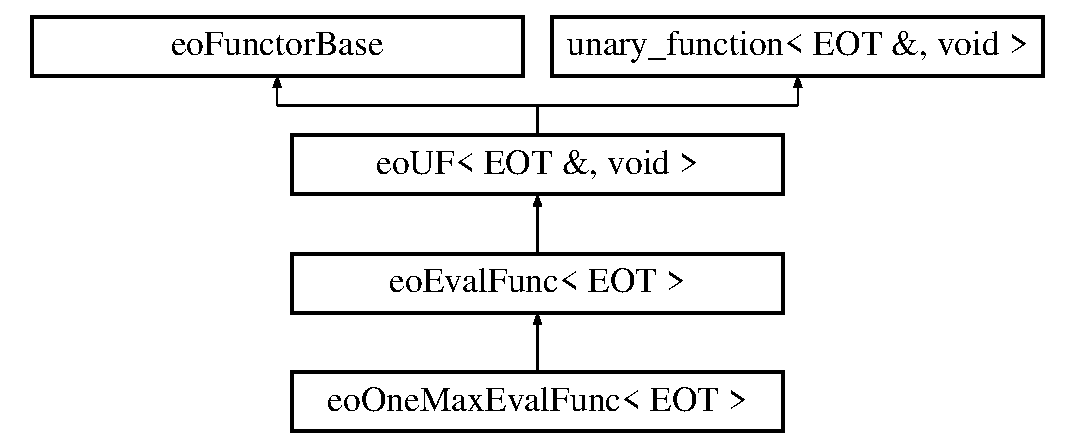
\includegraphics[height=4cm]{classeo_one_max_eval_func}
\end{center}
\end{figure}
\subsection*{Public Member Functions}
\begin{CompactItemize}
\item 
{\bf eo\-One\-Max\-Eval\-Func} ()\label{classeo_one_max_eval_func_a0}

\begin{CompactList}\small\item\em Ctor - no requirement. \item\end{CompactList}\item 
void {\bf operator()} ({\bf EOT} \&\_\-eo)
\begin{CompactList}\small\item\em Actually compute the fitness. \item\end{CompactList}\end{CompactItemize}


\subsection{Detailed Description}
\subsubsection*{template$<$class EOT$>$ class eo\-One\-Max\-Eval\-Func$<$ EOT $>$}

Always write a comment in this format before class definition if you want the class to be documented by Doxygen. 



Definition at line 26 of file eo\-One\-Max\-Eval\-Func.h.

\subsection{Member Function Documentation}
\index{eoOneMaxEvalFunc@{eo\-One\-Max\-Eval\-Func}!operator()@{operator()}}
\index{operator()@{operator()}!eoOneMaxEvalFunc@{eo\-One\-Max\-Eval\-Func}}
\subsubsection{\setlength{\rightskip}{0pt plus 5cm}template$<$class EOT$>$ void {\bf eo\-One\-Max\-Eval\-Func}$<$ {\bf EOT} $>$::operator() ({\bf EOT} \& {\em \_\-eo})\hspace{0.3cm}{\tt  [inline, virtual]}}\label{classeo_one_max_eval_func_a1}


Actually compute the fitness. 

\begin{Desc}
\item[Parameters:]
\begin{description}
\item[{\em EOT}]\& \_\-eo the {\bf EO}{\rm (p.\,\pageref{class_e_o})} object to evaluate it should stay templatized to be usable with any fitness type \end{description}
\end{Desc}


Implements {\bf eo\-UF$<$ EOT \&, void $>$} {\rm (p.\,\pageref{classeo_u_f_a1})}.

Definition at line 45 of file eo\-One\-Max\-Eval\-Func.h.

References EO$<$ F $>$::fitness(), and EO$<$ F $>$::invalid().

The documentation for this class was generated from the following file:\begin{CompactItemize}
\item 
eo\-One\-Max\-Eval\-Func.h\end{CompactItemize}
